\documentclass[]{standalone}

\usepackage{amsmath}
\usepackage{amsfonts}
\usepackage{amssymb}
\usepackage{graphicx}
\usepackage{tikz}
\usepackage{import}
\usepackage[subpreambles=true]{standalone}

\usepackage{tikz}
\usepackage{tikz-3dplot}
\usepackage{tikz_utils}

\usetikzlibrary{calc}
\usetikzlibrary{positioning}
\usetikzlibrary{patterns}
\usetikzlibrary{decorations,backgrounds}

\begin{document}
    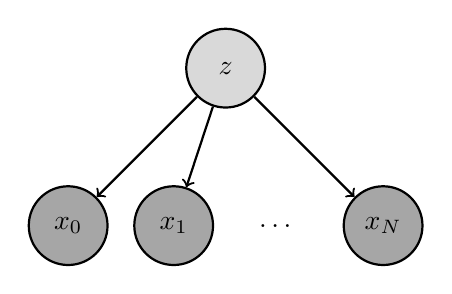
\begin{tikzpicture}[scale=1, thick]
        % unobserved
        \node (z) at (0,0) [shape=circle,draw=black, fill=gray!30, minimum size=1cm] {$z$};

        % observed
        \node (x0) at (-2,-2) [shape=circle,draw=black, fill=gray!70, minimum size=1cm] {$x_0$};
        \node (x1) at (-0.66,-2) [shape=circle,draw=black, fill=gray!70, minimum size=1cm] {$x_1$};
        \node (dots) at (0.66,-2) {\ldots};
        \node (xn) at (2,-2) [shape=circle,draw=black, fill=gray!70, minimum size=1cm] {$x_N$};
        \draw[->] (z) -- (x0);
        \draw[->] (z) -- (x1);
        \draw[->] (z) -- (xn);


        % \node (theta) at (0,2) [shape=circle,draw=red,fill=red, inner sep=0pt, minimum size=2mm,label=north:$\boldsymbol{\theta}$] {};
        % \node (sigma) at (2,2) [shape=circle,draw=red,fill=red, inner sep=0pt, minimum size=2mm,label=north:$\sigma^2$] {};
        % \node (x) at (-2,0) [shape=circle,draw=red,fill=red, inner sep=0pt, minimum size=2mm,label=west:$\mathbf{x}_n$] {};
        % \node (y) at (2,0) [shape=circle,draw=red,fill=blue!70, minimum size=10mm,label=south:$\mathbf{t}_n$] {};
        % \draw (theta) [->, red] -- (f);
        % \draw (x) [->, red] -- (f);
        % \draw (f) [->, red] -- (y);
        % \draw (sigma) [->, red] -- (y);
    \end{tikzpicture}
\end{document}